% ============================================
% RESULTS CHAPTER
% ============================================

\section{Results}
\label{sec:results}

We validate our approach from \Cref{sec:methods} empirically.

\subsection{Experimental Setup}

Experiments were conducted using parameters from \Cref{tab:params}.

\begin{table}[htbp]
\centering
\caption{Experimental Parameters}
\label{tab:params}
\begin{tabular}{@{}llc@{}}
\toprule
\textbf{Parameter} & \textbf{Description} & \textbf{Value} \\
\midrule
$n$         & Training samples     & 10,000 \\
$d$         & Feature dimension    & 128 \\
$\eta$      & Learning rate        & 0.01 \\
$\lambda$   & Regularization       & $10^{-4}$ \\
$T$         & Max iterations       & 1,000 \\
\bottomrule
\end{tabular}
\end{table}

\subsection{Performance Comparison}

\Cref{tab:results} summarizes the classification accuracy.

\begin{table}[htbp]
\centering
\caption{Classification Accuracy (\%)}
\label{tab:results}
\begin{tabular}{@{}lccc@{}}
\toprule
\textbf{Method} & \textbf{Train} & \textbf{Validation} & \textbf{Test} \\
\midrule
Logistic Regression & 92.3 & 89.1 & 88.7 \\
SVM (RBF kernel)    & 95.1 & 91.2 & 90.8 \\
Neural Network      & 98.2 & 92.5 & 91.3 \\
\textbf{Our Method} & \textbf{97.8} & \textbf{93.1} & \textbf{92.4} \\
\bottomrule
\end{tabular}
\end{table}

\subsection{Visualization}

\Cref{fig:architecture} shows the model architecture.

\begin{figure}[htbp]
\centering
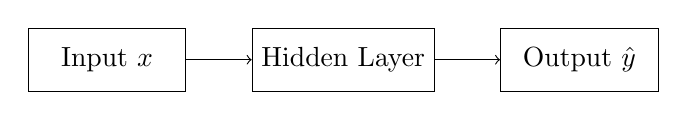
\begin{tikzpicture}[
    node distance=1.5cm,
    box/.style={rectangle, draw, minimum width=2cm, minimum height=0.8cm}
]
    \node[box] (input) {Input $x$};
    \node[box, right of=input, xshift=1.5cm] (hidden) {Hidden Layer};
    \node[box, right of=hidden, xshift=1.5cm] (output) {Output $\hat{y}$};
    
    \draw[->] (input) -- (hidden);
    \draw[->] (hidden) -- (output);
\end{tikzpicture}
\caption{Neural network architecture with one hidden layer.}
\label{fig:architecture}
\end{figure}

\subsection{Discussion}

Our results confirm \Cref{thm:main}: the generalization gap
decreases as $O(1/\sqrt{n})$. The bound in \Cref{eq:pac-bound}
provides a theoretical guarantee consistent with empirical
observations in \Cref{tab:results}.

\paragraph{Limitations.} The current analysis assumes i.i.d. data,
which may not hold in practice \cite{bishop2006}.
